\chapter{Literature Review}\doublespacing
\section{Data-Driven Control}
The foundation of data-driven control can be traced to the influential work in \cite{willems2005note} in the behavioral framework. Assuming that the given input is persistently exciting, suitable data-dependent matrices can describe the behavior of any LTI system. The papers \cite{Berberich2019a} and proven in \cite{Waarde2020} provided rigorous guarantees for system analysis and controller design using trajectories.

Data-Driven analysis methods can be categorised into three setups
\begin{itemize}
\item \cite{Wahlberg2010,Rojas2012,Tanemura2019,Romer2019c,Mueller2017} focusses on estimating properties using online sampling, by repeatedly choosing the input and measuring the output.
\item \cite{Montenbruck2016a,Romer2017a,Sharf2020,Romer2019b,Martin2020} focusses on analysing nonlinear systems using large amounts of input-output trajectories.
\item \cite{Maupong2017,Romer2019a,Koch2020,Koch2020a,Saeki2020} focusses on analysing LTI systems using a single input-state or input-output trajectory 
\end{itemize}
A limitation of all the methods is the requirement of direct access to plants and the need for more time due to the complexity of the approach.

Recent data-driven developments include state-feedback design \cite{Persis2020}, controller synthesis \cite{Berberich2019c}, dissipativity analysis \cite{Maupong2017,Romer2019a,Koch2020}, model predictive control \cite{Coulson2019,Berberich2019b} and data informativity \cite{8960476}.
\subsection{Dissipativity Analysis}
Willems' seminal papers \cite{Willems1972DissipativeDS,Willems1972DissipativeDS2} on dissipative dynamical systems introduced the concept of dissipativity. He reformulated the dissipation inequality as a linear matrix inequality.

Dissipativity properties facilitate system analysis and application of feedback theorems ensuring closed-loop stability. \cite{Zames1966,Schaft2000} includes the standard feedback theorems and controller design based on dissipativity properties which has led to numerous approaches for determining such properties from data.

\paragraph{Transition to the Discrete Framework}
Willems recognised the limitations of the input-output framework, leading to the development of the behavioral theory. Willems introduced the concept of quadratic differential forms (QDF) which are used to represent supply rates and storage functions for any dissipative system \cite{Trentelman1997}. \cite{Maupong2017} introduced another notion of L-dissipativity for finite-horizon cases.

\subsection{Informativity Approach}
Recently, there has been significant interest in inferring dissipativity properties from data.
The informativity approach bounds the noise by a quadratic matrix inequality (QMI). It determines whether \emph{all} systems satisfying such QMI are dissipative. This approach has its similarities with robust-control \cite{Megretski1997, Iwasaki1998, Scherer1997,Scherer2001}. But here, data is directly mapped to storage functions. 
\section{Other Data-Driven Approaches}
Though we will be focussing on the informativity approach, let us also discuss other data-driven approaches in some detail.
\subsection{Dynamic Mode Decomposition}

Dynamic Mode Decomposition (DMD) offers an operator-theoretic perspective based on system measurement evolution, complementing classical geometric and statistical perspectives on control systems. An example is Koopman operator theory \cite{brunton2021modern}, which represents nonlinear dynamics using intrinsic coordinate systems of a linear framework, exploiting the low-dimensional behavior of many real-life infinite-dimensional dynamical systems.

It decomposes the system into various modes where each mode consists of spatially correlated structures exhibiting the same linear behavior in time, i.e. the same characteristic value of $\lambda = a + ib$, where $a$ represents the growth rate and $b$ is the oscillation frequency. DMD also models the evolution of each mode over time, utilizing the computationally efficient singular value decomposition (SVD) to calculate these modes. DMD is fundamentally data-driven, as no knowledge of governing equations is required and the results are applicable to both experimental and numerical data. It has various variants applicable to existing system identification and modal extraction techniques. An example of DMD applied to fluid flow is shown in Figure \ref{fig
}.

\begin{figure}[!hbt]
\centering
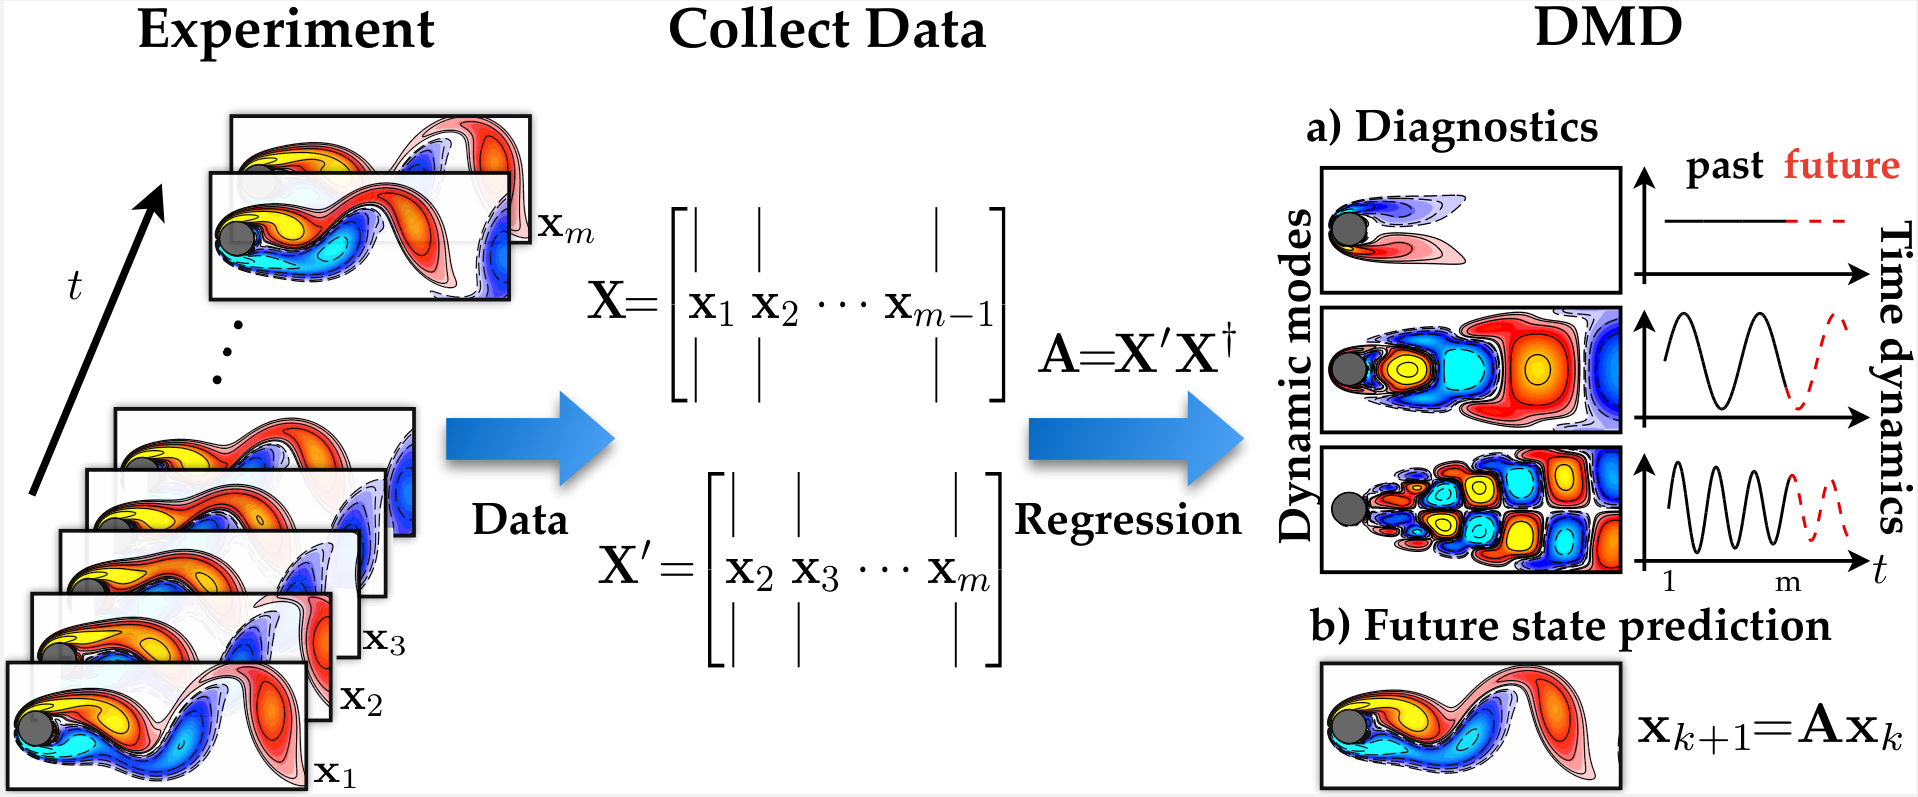
\includegraphics[width=\linewidth]{Images/fig3p1.png}
\caption{\cite{dmdkutz}, Overview of DMD, using fluid flow past a circular cylinder}
\label{fig
}
\end{figure}

\subsubsection{Extensions, Applications and Limitations}
\begin{description}
\item[Including inputs and control] Proctor \cite{proctor2014dynamic} introduced Dynamic Mode Decomposition with Control (DMDc) for the design of effective controllers using data.
\item[Compression and randomized linear algebra] Randomized DMD algorithms \cite{Erichson2019} work more efficiently by projecting data onto lower-dimensional subspaces. \emph{Sparsity} can also be utilised for efficient measurements \cite{brunton2021modern}.
\item[Multiresolution] multi-resolution Dynamic Mode Decomposition (mrDMD) \cite{kutz2015multiresolution} accurately captures dynamics with different timescales such as El Ni\~no.
\item[Epidemiology] Proctor and Eckhoff \cite{Proctor2015DiscoveringDP} provided interpretable decompositions for data consisting of high-dimensional spatiotemporal time series measurements, such as the number of infections in a given neighbourhood or city. 
\item[Strong Nonlinearity] DMD struggles to capture systems with nonlinear features such as chaos and multiple fixed points. Sparse Identification of Nonlinear Dynamics (SINDy) \cite{SINDy} is better at identifying nonlinear systems but it has it own limitations.
\end{description}
\begin{comment}
DMD's extensions and connections with other data-driven techniques, have led to multiple implementation techniques. These include fast DMD (optimized using randomized linear algebra) and multi-resolution DMD (splitting data into sequential snapshots to capture multi-scale behavior).

\subsubsection{Dynamic Mode Decomposition with Control}
Dynamic Mode Decomposition with Control (DMDc) modifies DMD to account for input influence, enabling identification of how external forcing impacts a system and how actuators influence different dynamic modes. DMDc combines the advantages of system identification and dimensionality reduction, offering a balance between model complexity and computational efficiency.

\subsection{System Identification with the Koopman Operator}
% In recent years, there has been significant interest in leveraging the Koopman operator for data-driven analysis of complex systems. 
The Koopman operator maps the state space of nonlinear systems into a higher-dimensional space of a linear system. This linear perspective enables easier and effective analysis and behavior prediction of complex dynamical systems. %through a linear perspective by mapping the state space into a higher-dimensional space where the dynamics can be represented linearly. This approach has been particularly effective in understanding and predicting the behavior of systems with complex, nonlinear dynamics.

% \subsubsection{Koopman Operator Theory}
Koopman Operator achieves this by relying on the evolution of observables which are functions of the state instead of relying on the evolution of state variables. The Koopman operator $\mathcal{K}$ for a dynamical system $\dot{x} = f(x)$, acts on an observable $g(x)$, giving the expression $\mathcal{K}g(x) = g(f(x))$.
% The advantage of this approach is that it transforms the nonlinear problem into a linear one, albeit in an infinite-dimensional space of observables.

\paragraph{Data-Driven Koopman Operator Approximations}

Given some data, we can approximate the Koopman operator by identifying a finite-dimensional subspace of observables that captures the essential dynamics of the system using the below techniques:
%This can be achieved through various methods, including Extended Dynamic Mode Decomposition (EDMD) and Neural Network-based approaches.

\subsubsection{Extended Dynamic Mode Decomposition (EDMD)}
Here, the traditional DMD framework is extended by incorporating a more observables, allowing for more accurate representation of the Koopman operator. Then, the Koopman operator can be represented as a matrix approximation based on the data and selected observables.% EDMD has been successfully applied to a wide range of systems, demonstrating its versatility and effectiveness.

\subsubsection{Neural Network-based Approaches}

Recent advancements in machine learning have spurred the development of neural network-based methods for approximating the Koopman operator. These methods learn the appropriate observables directly from data by leveraging the features of neural networks. Techniques such as Deep Koopman and Variational Koopman have shown promise in capturing the dynamics of complex, high-dimensional systems.
\section{Applications}
Here, we mention several case studies that demonstrate the effectiveness of data-driven control and system identification in real-world scenarios.

\subsection{Fluid Dynamics}

In fluid dynamics, data-driven methods have been employed to analyse and control complex flow patterns. For instance, these techniques have been used to identify coherent structures in turbulent flows, predict vortex shedding, and design control strategies for reducing drag in aerodynamic systems.

\subsection{Robotics}

Robotics is another field where data-driven control has made significant strides. Techniques such as reinforcement learning, combined with Koopman operator-based models, have enabled the development of robust controllers for high-dimensional robotic systems. These approaches facilitate tasks such as trajectory planning, obstacle avoidance, and dynamic manipulation.

\subsection{Power Systems}

In power systems, these methods are used for system identification, fault detection, and stability analysis. For example, DMD has been applied to identify oscillatory modes in power grids, enabling the design of controllers that enhance system stability and resilience to disturbances.

\subsection{Biomedical Engineering}

Biomedical engineering has also benefited from such approaches. Techniques like EDMD and neural network-based Koopman operators can model and control biological systems, such as glucose-insulin dynamics in diabetes management and neural activity in brain-machine interfaces.

\end{comment}
\subsection{Sparse Identification of Nonlinear Dynamics (SINDy)}
Discovering dynamical systems models from data has always been a central challenge in modelling systems, going back to the time when Kepler and Newton discovered the laws of planetary motion. The automated discovery of governing equations is a new and exciting paradigm with increasing computational power and vast data.
 
The sparse identification of nonlinear dynamics (SINDy) algorithm \cite{SINDy} bypasses the intractable combinatorial search through all possible model structures, and uses the fact that many dynamical systems have dynamics $\bf$ with only a few active terms in the space of possible right-hand side functions as shown in \ref{fig:sindydemo}.

This has been possible due to recent advances in compressed sensing and sparse regression. It also allows the dynamics to vary concerning bifurcation parameters $\bmuu\in\mathbb{R}^q$.  
\begin{figure}[H]
    \centering
    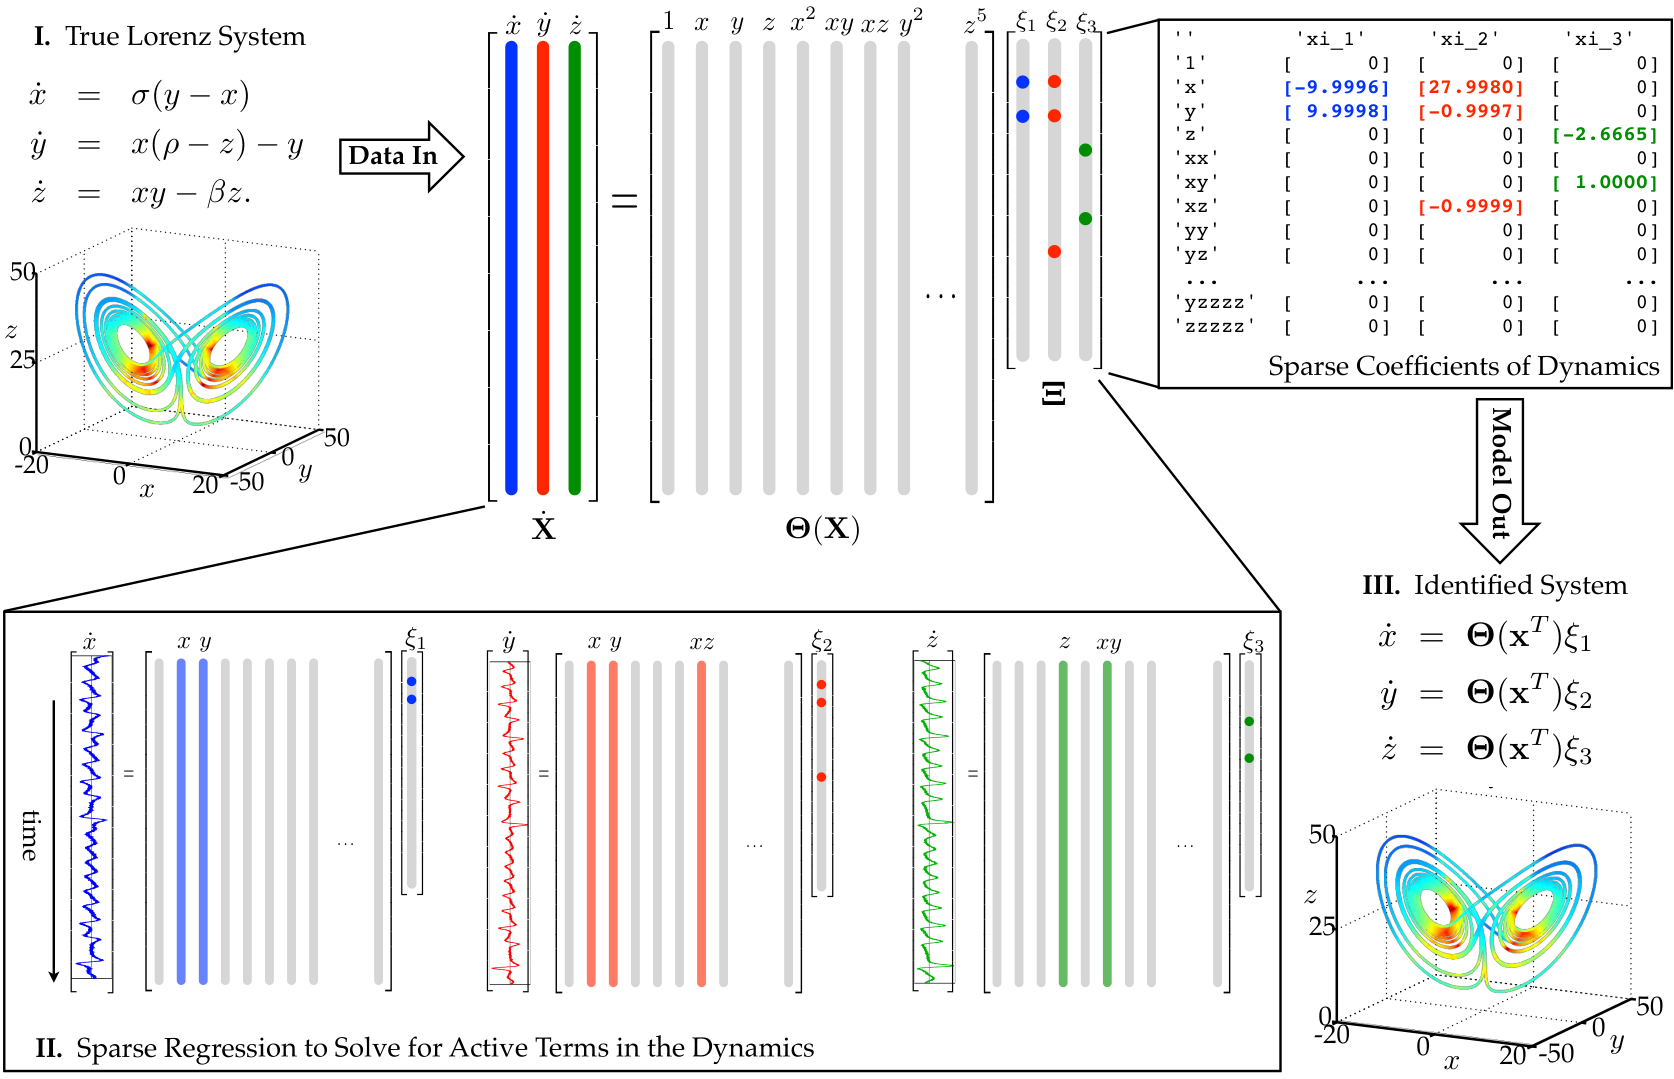
\includegraphics[width=\linewidth]{Images/FIG00_BIG4.png}
    \caption{\cite{SINDy}, Overview of SINDy, using the Lorenz equations}
    \label{fig:sindydemo}
\end{figure}
\subsubsection{Extensions, Applications and Limitations}
\begin{description}
    % \item[Normal Forms, Bifurcations, and Parameterized Systems]
    \item[Constrained sparse Galerkin regression] Loiseau and Brunton \cite{loiseau2016constrained} generalised the SINDy framework to incorporate known physical constraints and symmetries in the equations by implementing a constrained sequentially thresholded least-squares optimization by imposing energy-preserving constraints on the quadratic nonlinearities in the Navier–Stokes equations.
    \item[Rational Function Nonlinearities] Kaheman \cite{Kaheman2020} reformulated the dynamics in an implicit ordinary differential equation (ODE) and modified the optimization procedure to work for rational functions which are not a sparse linear combination of few basis functions. Such rational function nonlinearities occur in metabolic and regulatory networks in biology.
    \item[Implicit ODEs] The optimization procedure above may be generalized to include a larger class of implicit ordinary differential equations in addition to those containing rational function nonlinearities. This can be achieved by updating our library of functions.
    \item[Limitations] Linear and Nonlinear Disambiguation Optimization (LANDO) \cite{Baddoo2022} resolves scaling issues for systems not inhibiting low-dimensional subspace by using kernels for learning representations \cite{brunton2021modern}.
\end{description}
\section{Attacks on Data-Driven Control}
A popular security measure is to focus on knowledge of explicit models against attacks such as zero-dynamics attacks~\cite{Pasqualetti2015Control}, observer-based attacks~\cite{Giraldo2018A}, and moving target defence~\cite{Griffioen2020Moving}.
Nowadays, approaches using data-driven attack detection~\cite{Krishnan2020Data} and stealthy design~\cite{Alisic2021Data,Alisic2023Model} are also being utilised.
\clearpage
\section{Conclusion}
Data-driven approaches represent a paradigm shift in the analysis and control of complex dynamical systems. By leveraging data to directly infer system properties and design controllers, these techniques offer a powerful alternative to traditional model-based approaches. 
However, the vulnerability of data-driven control algorithm has received less attention, and there is a need for dedicated techniques to address this issue which will be addressed in this report.
% Future research directions include the development of more efficient algorithms, integration with real-time control systems, and application to increasingly complex and high-dimensional systems. The continued advancement of data-driven methods promises to unlock new possibilities in a wide range of scientific and engineering domains.